%%%%%%%%%%%%%%%%%%%%%%%%%%%%%%%%%%%%%%%%%%%%%%%%%%%%%%%%%%%%%%%%%%%%%%%%%%%%%%%
%%%%%%%%%%%%%%%%%%%%%%%%%%%%%%%%%%%%%%%%%%%%%%%%%%%%%%%%%%%%%%%%%%%%%%%%%%%%%%%
% APPENDIX
%%%%%%%%%%%%%%%%%%%%%%%%%%%%%%%%%%%%%%%%%%%%%%%%%%%%%%%%%%%%%%%%%%%%%%%%%%%%%%%
%%%%%%%%%%%%%%%%%%%%%%%%%%%%%%%%%%%%%%%%%%%%%%%%%%%%%%%%%%%%%%%%%%%%%%%%%%%%%%%
% \newpage
\appendix
% \onecolumn
\section{Additional Results}

\subsection{Training Dynamics}
\begin{figure}[htbp]
\centering

% Row 1
\begin{subfigure}{\textwidth}
    \centering
    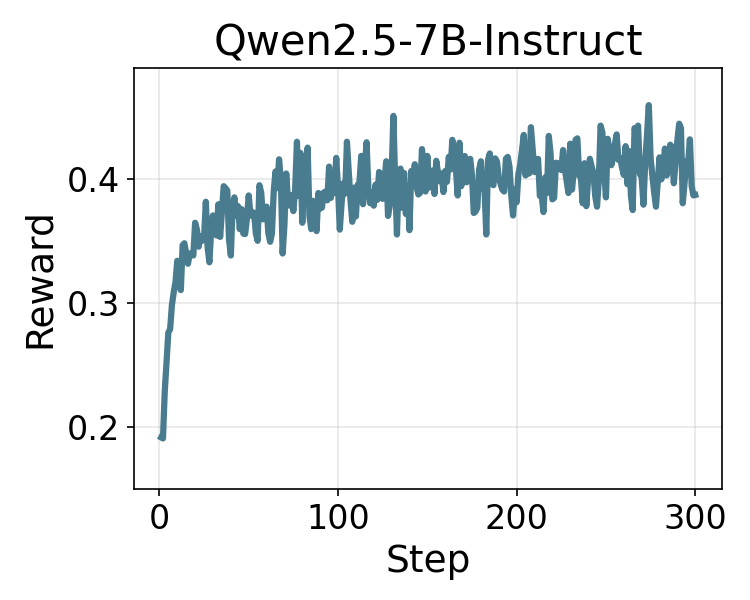
\includegraphics[width=0.3\textwidth]{img/rl_training_reward_EM_qwen2.5-7b-instruct.png}
    \hfill
    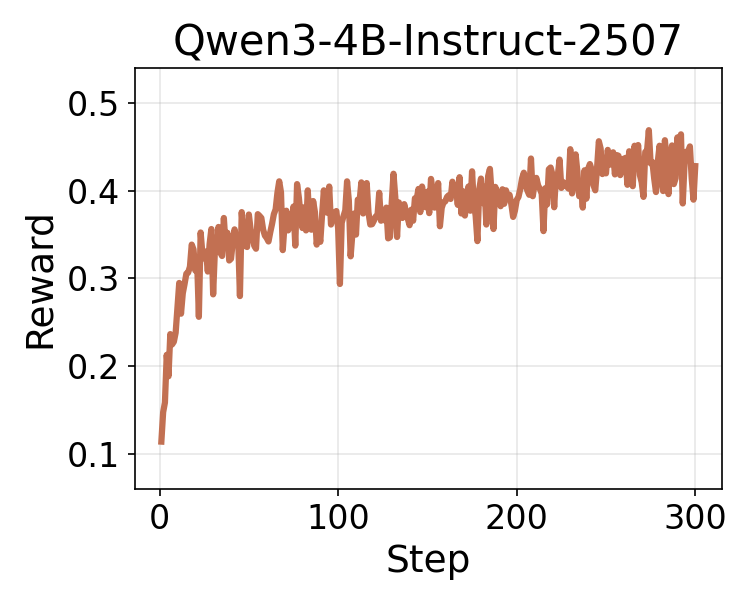
\includegraphics[width=0.3\textwidth]{img/rl_training_reward_EM_qwen3-4b-instruct-2507.png}
    \hfill
    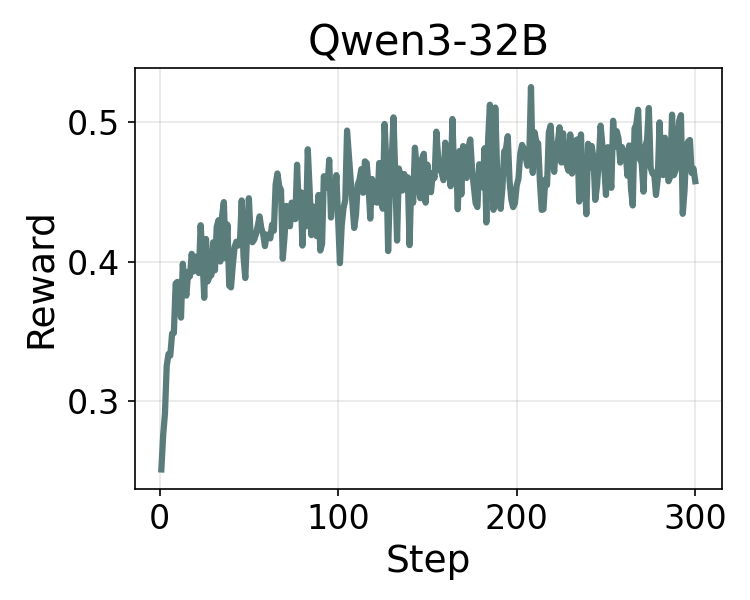
\includegraphics[width=0.3\textwidth]{img/rl_training_reward_EM_qwen3-32b.png}
    \caption{Search-R1}
\end{subfigure}

\vspace{0.5em}

% Row 2
\begin{subfigure}{\textwidth}
    \centering
    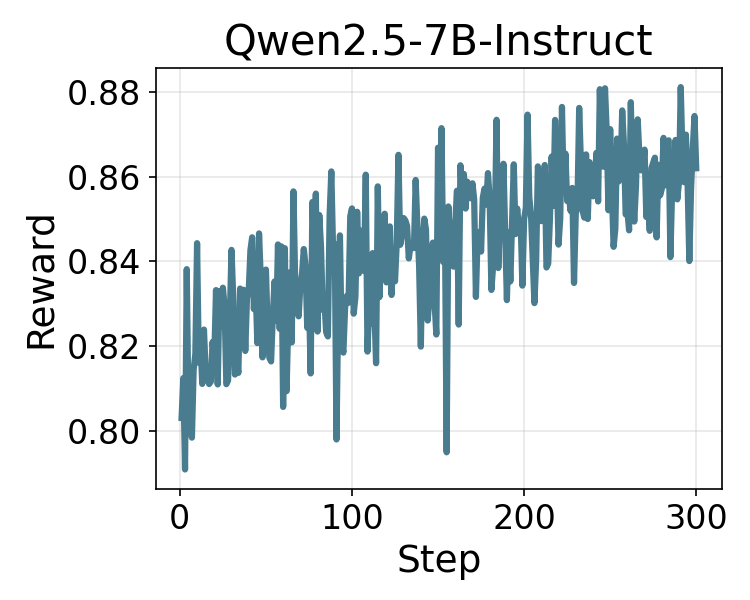
\includegraphics[width=0.3\textwidth]{img/rl_training_reward_CJ_qwen2.5-7b-instruct.png}
    \hfill
    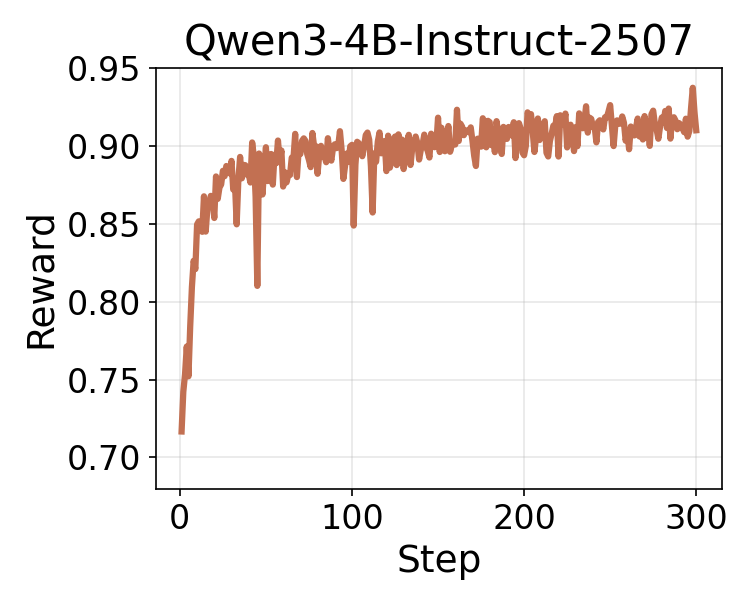
\includegraphics[width=0.3\textwidth]{img/rl_training_reward_CJ_qwen3-4b-instruct-2507.png}
    \hfill
    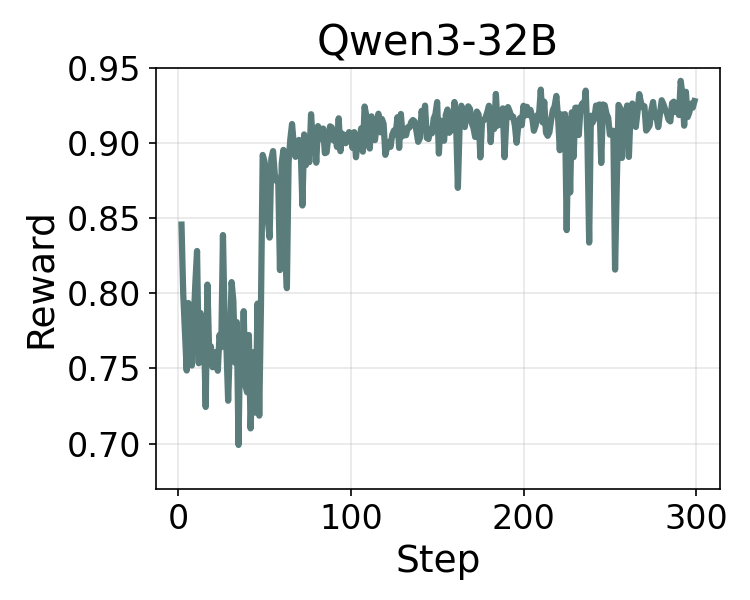
\includegraphics[width=0.3\textwidth]{img/rl_training_reward_CJ_qwen3-32b.png}
    \caption{Constitutional Judge (CJ)}
\end{subfigure}

\vspace{0.5em}

% Row 3
\begin{subfigure}{\textwidth}
    \centering
    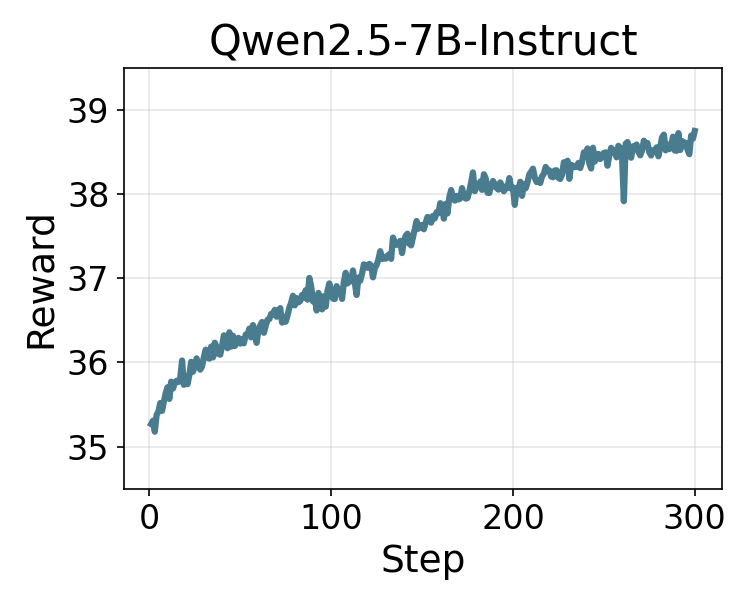
\includegraphics[width=0.3\textwidth]{img/rl_training_reward_RLIF_qwen2.5-7b-instruct.png}
    \hfill
    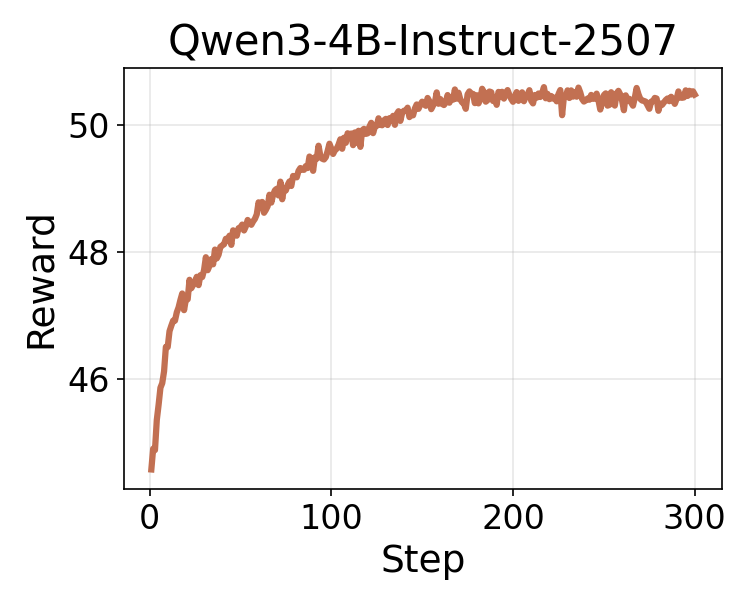
\includegraphics[width=0.3\textwidth]{img/rl_training_reward_RLIF_qwen3-4b-instruct-2507.png}
    \hfill
    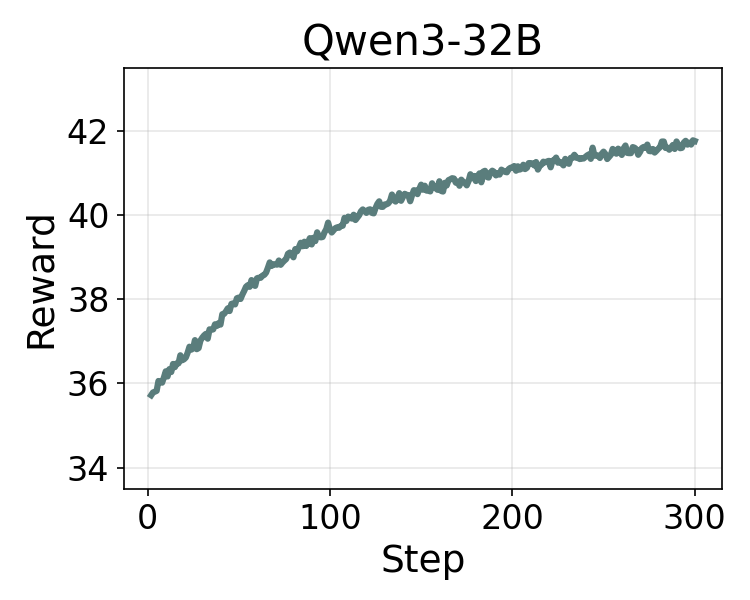
\includegraphics[width=0.3\textwidth]{img/rl_training_reward_RLIF_qwen3-32b.png}
    \caption{RLIF}
\end{subfigure}

\vspace{0.5em}

% Row 4
\begin{subfigure}{\textwidth}
    \centering
    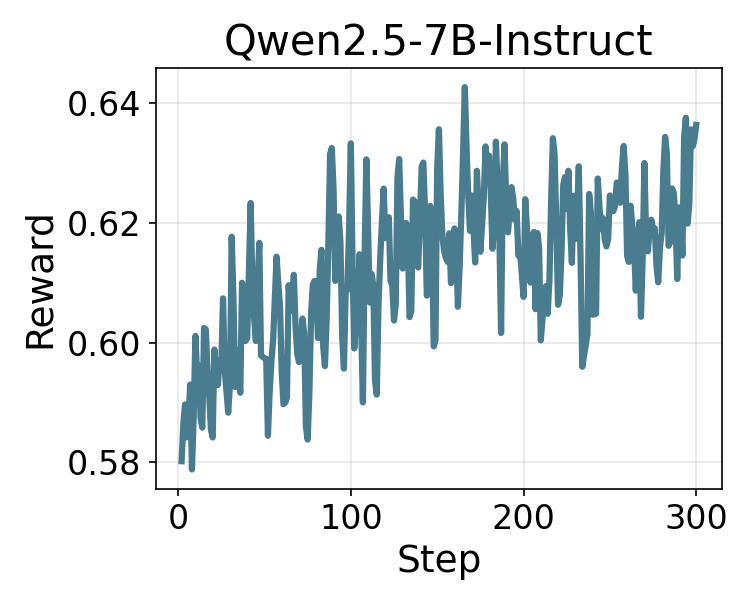
\includegraphics[width=0.3\textwidth]{img/rl_training_reward_CCS_qwen2.5-7b-instruct.png}
    \hfill
    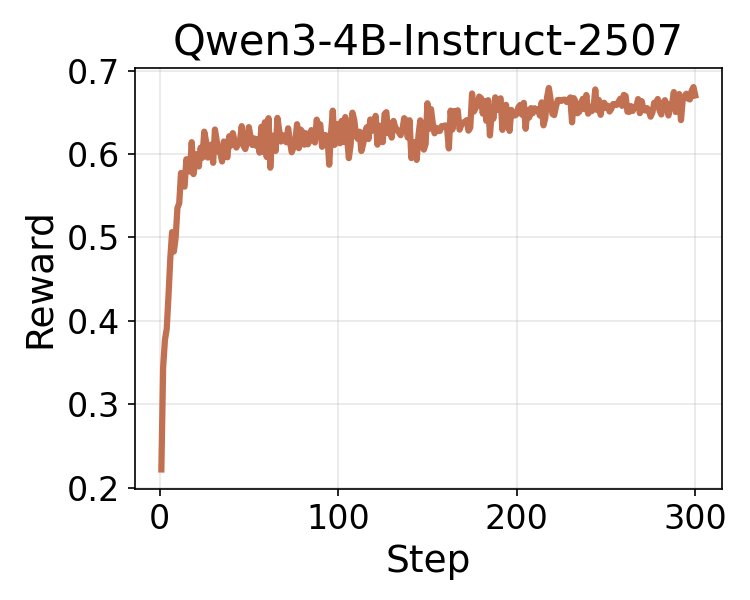
\includegraphics[width=0.3\textwidth]{img/rl_training_reward_CCS_qwen3-4b-instruct-2507.png}
    \hfill
    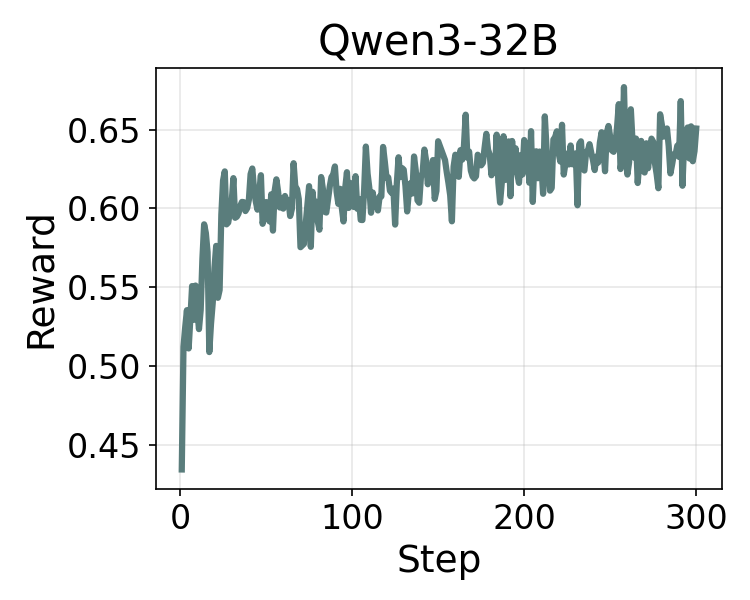
\includegraphics[width=0.3\textwidth]{img/rl_training_reward_CCS_qwen3-32b.png}
    \caption{CCS}
\end{subfigure}

\caption{\textbf{Training Reward during RL.}}
\label{fig:rl_train_reward}

\end{figure}
% \begin{figure}[htbp]
% \centering

% \begin{subfigure}{0.3\textwidth}
% \centering
% 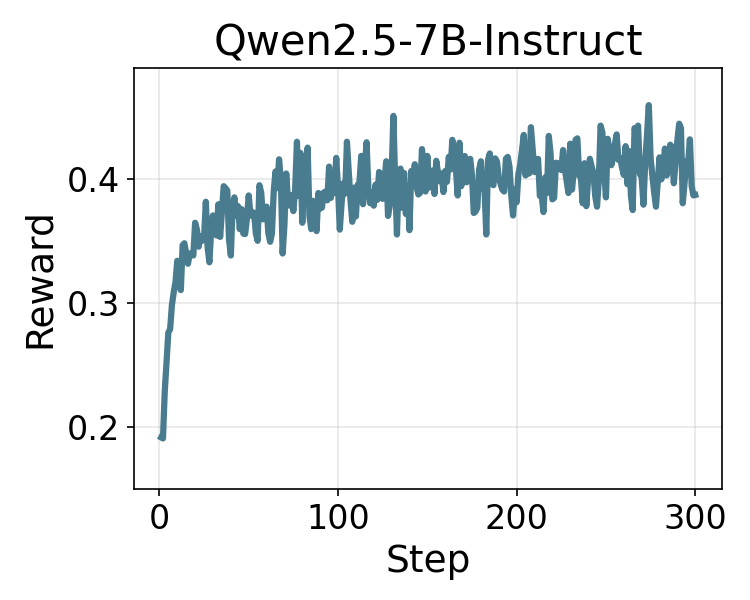
\includegraphics[width=\linewidth]{img/rl_training_reward_EM_qwen2.5-7b-instruct.png}
% \end{subfigure}
% \hfill
% \begin{subfigure}{0.3\textwidth}
% \centering
% 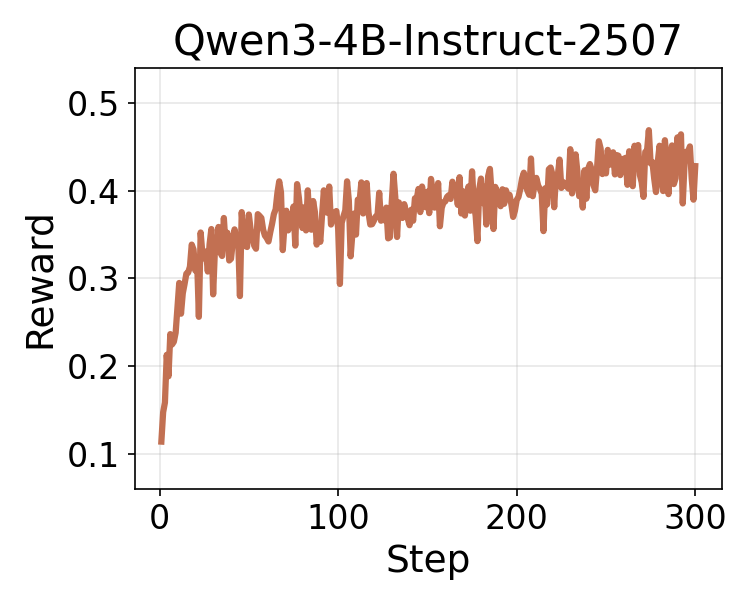
\includegraphics[width=\linewidth]{img/rl_training_reward_EM_qwen3-4b-instruct-2507.png}
% \end{subfigure}
% \hfill
% \begin{subfigure}{0.3\textwidth}
% \centering
% 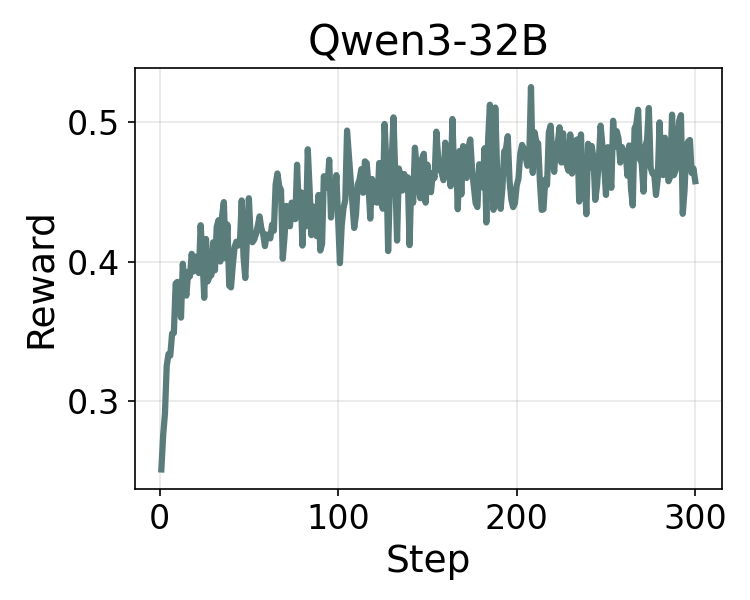
\includegraphics[width=\linewidth]{img/rl_training_reward_EM_qwen3-32b.png}
% \end{subfigure}

% \begin{subfigure}{0.3\textwidth}
% \centering
% 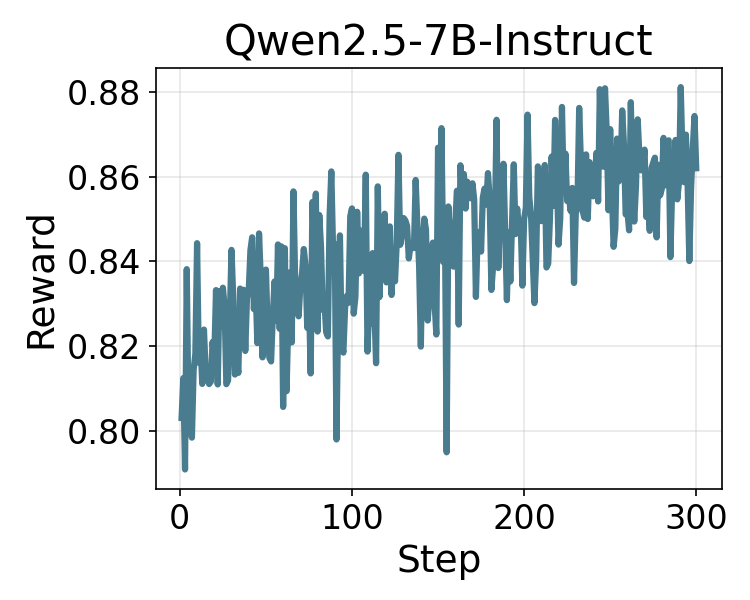
\includegraphics[width=\linewidth]{img/rl_training_reward_CJ_qwen2.5-7b-instruct.png}
% \end{subfigure}
% \hfill
% \begin{subfigure}{0.3\textwidth}
% \centering
% 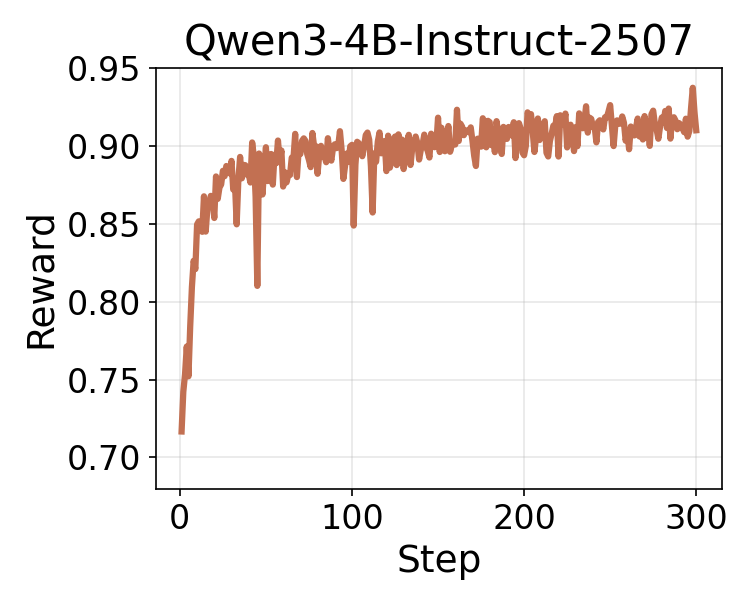
\includegraphics[width=\linewidth]{img/rl_training_reward_CJ_qwen3-4b-instruct-2507.png}
% \end{subfigure}
% \hfill
% \begin{subfigure}{0.3\textwidth}
% \centering
% 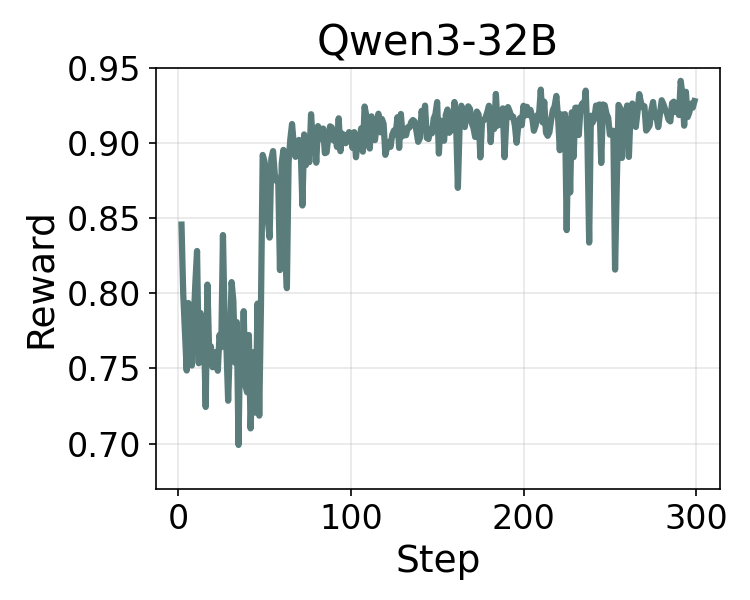
\includegraphics[width=\linewidth]{img/rl_training_reward_CJ_qwen3-32b.png}
% \end{subfigure}

% \begin{subfigure}{0.3\textwidth}
% \centering
% 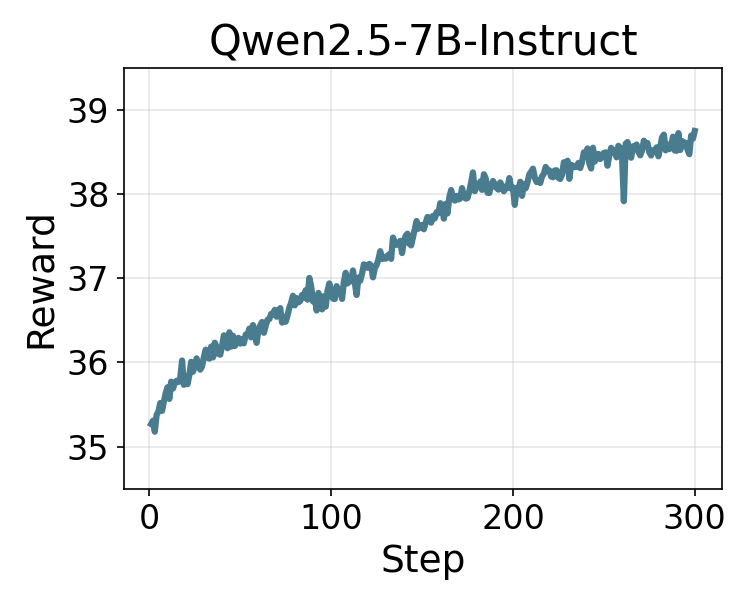
\includegraphics[width=\linewidth]{img/rl_training_reward_RLIF_qwen2.5-7b-instruct.png}
% \end{subfigure}
% \hfill
% \begin{subfigure}{0.3\textwidth}
% \centering
% 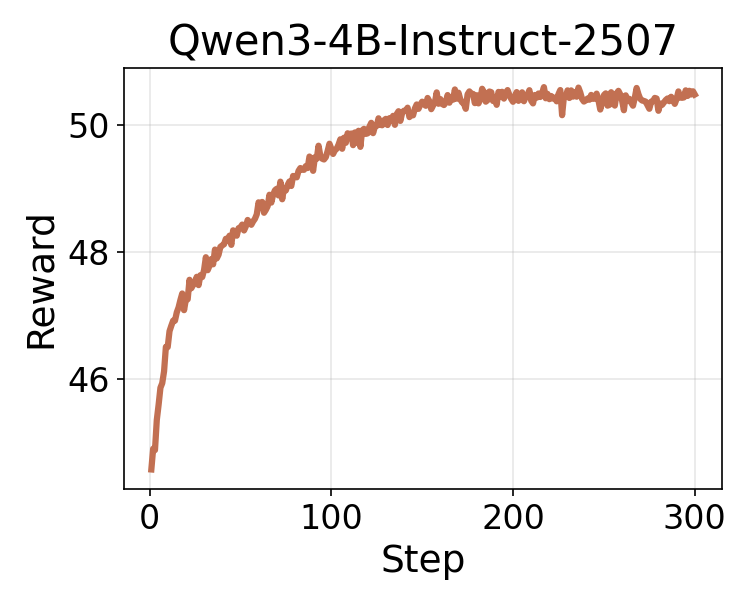
\includegraphics[width=\linewidth]{img/rl_training_reward_RLIF_qwen3-4b-instruct-2507.png}
% \end{subfigure}
% \hfill
% \begin{subfigure}{0.3\textwidth}
% \centering
% 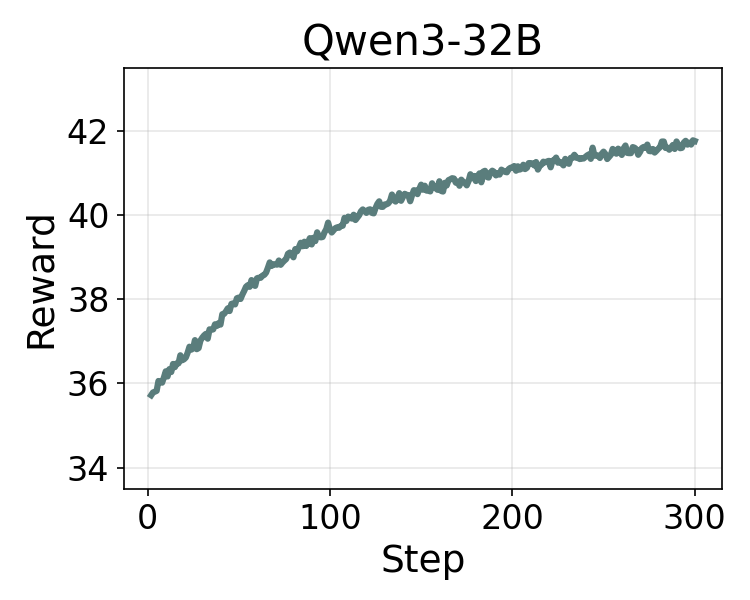
\includegraphics[width=\linewidth]{img/rl_training_reward_RLIF_qwen3-32b.png}
% \end{subfigure}

% \begin{subfigure}{0.3\textwidth}
% \centering
% 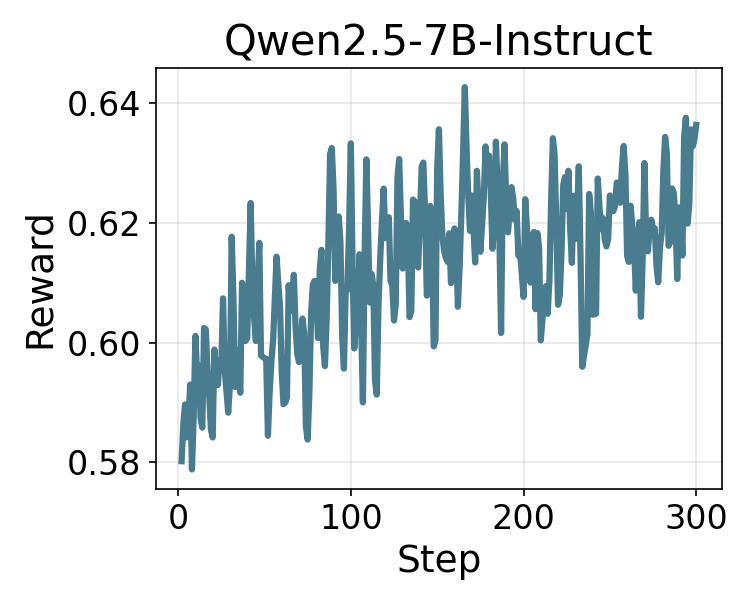
\includegraphics[width=\linewidth]{img/rl_training_reward_CCS_qwen2.5-7b-instruct.png}
% \end{subfigure}
% \hfill
% \begin{subfigure}{0.3\textwidth}
% \centering
% 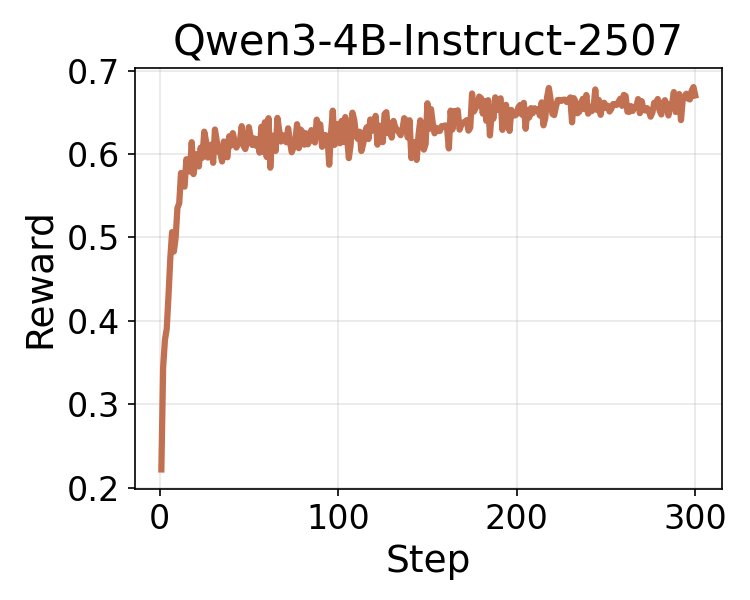
\includegraphics[width=\linewidth]{img/rl_training_reward_CCS_qwen3-4b-instruct-2507.png}
% \end{subfigure}
% \hfill
% \begin{subfigure}{0.3\textwidth}
% \centering
% 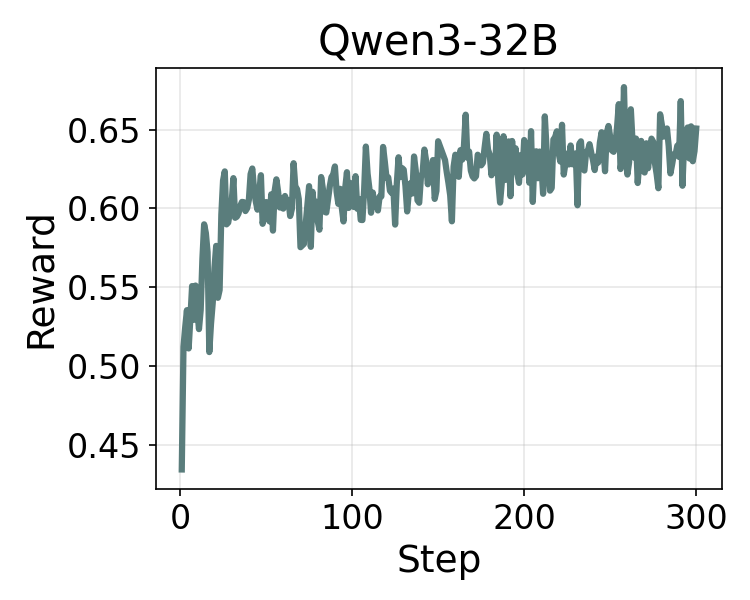
\includegraphics[width=\linewidth]{img/rl_training_reward_CCS_qwen3-32b.png}
% \end{subfigure}

% \caption{\textbf{Training Reward during RL.}}
% \label{fig:rl_train_reward}

% \end{figure}

We plot the training rewards of Search-R1, Constitutional Judge (CJ), RLIF, and CCS in \Cref{fig:rl_train_reward}. Since each method uses a different reward function and therefore operates on a different scale, we present them in separate plots. Additionally, the average number of searches is plotted in \Cref{fig:rl_avg_num_search}.


\begin{figure}[htbp]
\centering

\begin{subfigure}{0.32\textwidth}
\centering
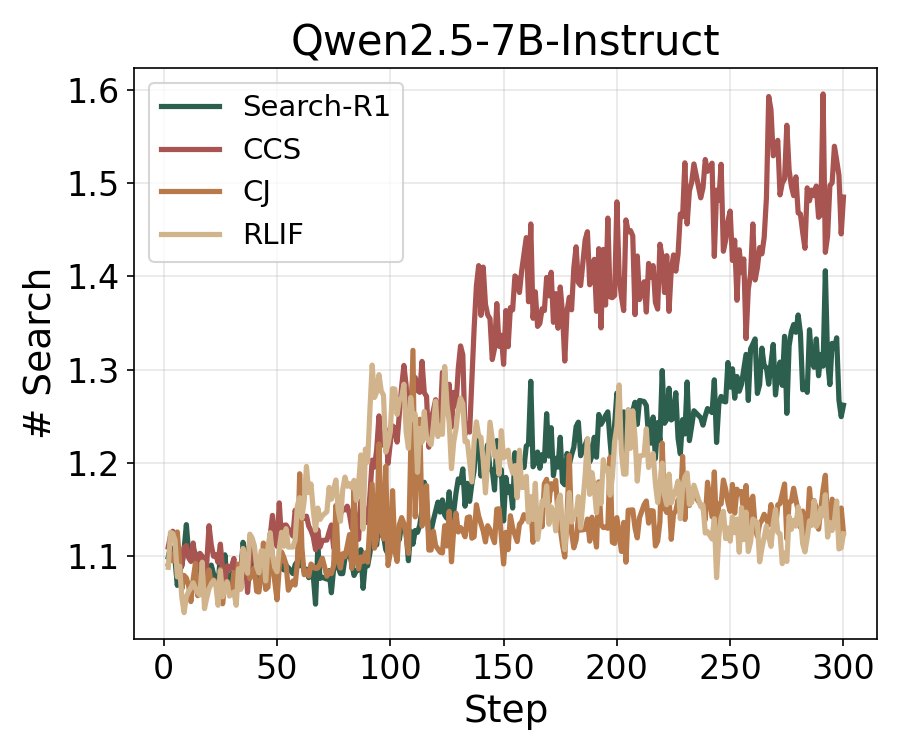
\includegraphics[width=\linewidth]{img/rl_avg_num_search_qwen2.5-7b-instruct.png}
\end{subfigure}
\hfill
\begin{subfigure}{0.32\textwidth}
\centering
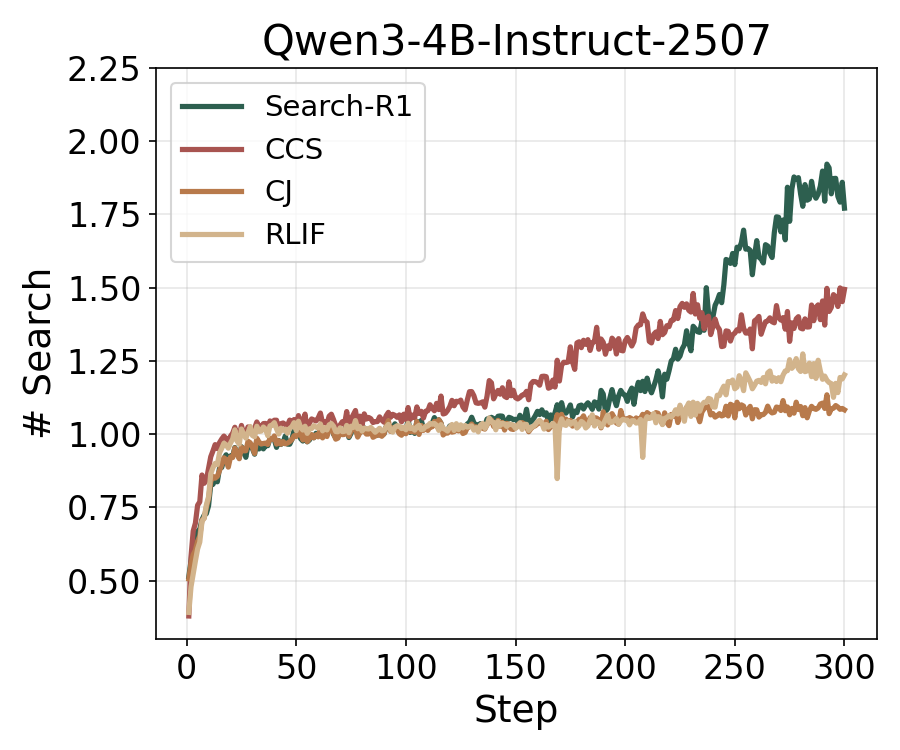
\includegraphics[width=\linewidth]{img/rl_avg_num_search_qwen3-4b-instruct-2507.png}
\end{subfigure}
\hfill
\begin{subfigure}{0.32\textwidth}
\centering
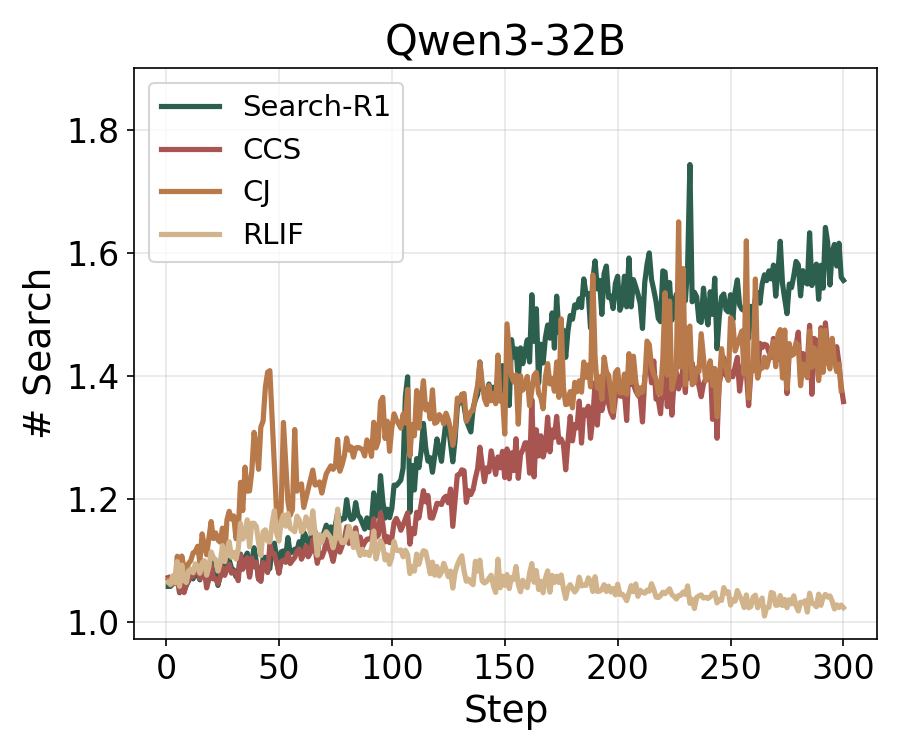
\includegraphics[width=\linewidth]{img/rl_avg_num_search_qwen3-32b.png}
\end{subfigure}

\caption{\textbf{Average number of search during RL.}}
\label{fig:rl_avg_num_search}

\end{figure}


% \subsection{Different Reconstructors}

\section{Implementation Details}
\label{appendix:implementaion_details}

\subsection{Hyperparameters}
\label{appendix:hyperparams}
We conduct experiments using three policy models: Qwen2.5-7B-Instruct, Qwen3-4B-Instruct-2507, and Qwen3-32B \citep{yang2025qwen3}. We use Gemini 2.5 Flash \citep{comanici2025gemini} as both the evaluator and reconstructor. We use Qwen3-Embedding-4B \citep{qwen3embedding} to compute the semantic similarity between $q$ and $\hat{q}$ in \Cref{eq:embedding_sim}, and bert-base-NER \citep{bert-base-NER} to mask search actions.

Following \citet{search-r1}, we train all fine-tuning-based baselines, including SFT and RL methods, on the merged training sets of NQ and HotpotQA. We evaluate the models on the test or validation splits of seven datasets to assess both in-domain and out-of-domain generalization. For evaluation, we use Gemini 2.5 Flash as the evaluator with the prompt described in \Cref{appendix:evaluator_prompt}. The evaluation temperature is set to 0.1.

For RL-based methods, we set the policy learning rate to $1\times10^{-6}$ and sample five responses per prompt. Training is performed for 300 steps using the FSDP2 strategy, with gradient checkpointing enabled to improve GPU memory efficiency.

All training runs are conducted on four nodes, each equipped with eight H100 GPUs. We use a total batch size of 512, a mini-batch size of 256, and a micro-batch size of 64 for Qwen2.5-7B-Instruct and Qwen3-4B-Instruct-2507. For Qwen3-32B, we use a micro-batch size of 32 due to memory constraints. The maximum context length is set to 30,000 tokens. The maximum response length for each step is 512 tokens, and the maximum search response length for each step is 8,192 tokens.

For efficient rollout generation, we use vLLM \citep{vllm} with tensor parallelism of size 1 for Qwen2.5-7B-Instruct and Qwen3-4B-Instruct-2507, and size 2 for Qwen3-32B. During rollout sampling, the temperature is set to 1.0 and top-$p$ is set to 1.0. The KL divergence regularization coefficient $\beta$ and the clip ratio $\epsilon$ are set to 0.01 and 0.2, respectively. The maximum action budget is set to 4, and up to 10 snippets are retrieved from the search engine.

\newpage
\subsection{Evaluation}
\label{appendix:evaluator_prompt}

% \newpage
\begin{promptbox}[]
Your job is to look at a question, a gold target, and a predicted answer, and then assign a grade of either ["CORRECT", "INCORRECT", "NOT_ATTEMPTED"].
First, I will give examples of each grade, and then you will grade a new example.


The following are examples of CORRECT predicted answers.
```
Question: What are the names of Barack Obama's children?
Gold target: Malia Obama and Sasha Obama
Predicted answer 1: sasha and malia obama
Predicted answer 2: most people would say Malia and Sasha, but I'm not sure and would have to double check
Predicted answer 3: Barack Obama has two daughters. Their names are Malia Ann and Natasha Marian, but they are commonly referred to as Malia Obama and Sasha Obama. Malia was born on July 4, 1998, and Sasha was born on June 10, 2001.
```
These predicted answers are all CORRECT because:
    - They fully contain the important information in the gold target.
    - They do not contain any information that contradicts the gold target.
    - Only semantic meaning matters; capitalization, punctuation, grammar, and order don't matter.
    - Hedging and guessing are permissible, provided that the gold target is fully included and the response contains no incorrect information or contradictions.


The following are examples of INCORRECT predicted answers.
```
Question: What are the names of Barack Obama's children?
Gold target: Malia and Sasha
Predicted answer 1: Malia.
Predicted answer 2: Malia, Sasha, and Susan.
Predicted answer 3: Barack Obama does not have any children.
Predicted answer 4: I think it's either Malia and Sasha. Or it could be Malia and Jackie. Or it could be Joey and Malia.
Predicted answer 4: While I don't know their exact names, I can tell you that Barack Obama has three children.
Predicted answer 5: It's possible you may mean Betsy and Olivia. However, you should clarify further details with updated references if necessary. Is that the correct answer?
Predicted answer 6: It may be the case that Obama's child is named James. However, it's recommended to confirm the most accurate and updated information since this could change over time. This model may not always reflect the most current information.
```
These predicted answers are all INCORRECT because:
    - A factual statement in the answer contradicts the gold target. Incorrect statements that have some hedging (e.g., "it is possible that", "although i'm not sure, i think") are also considered incorrect.


The following are examples of NOT_ATTEMPTED predicted answers.
```
Question: What are the names of Barack Obama's children?
Gold target: Malia and Sasha
Predicted answer 1: I don't know.
Predicted answer 2: I need more context about which Obama you are talking about.
Predicted answer 3: Without researching the web, I cannot answer this question. However, I can tell you that Barack Obama has two children.
Predicted answer 4: Barack Obama has two children. I know that one of them is Malia, but I'm not sure about the other one.
```
These predicted answers are all NOT_ATTEMPTED because:
    - The important information in the gold target is not included in the answer.
    - No statements in the answer contradict the gold target.


Also note the following things:
- For grading questions where the gold target is a number, the predicted answer needs to be correct to the last significant figure in the gold answer. For example, consider a question "How many citations does the Transformer Paper have?" with gold target "120k".
    - Predicted answers "120k", "124k", and 115k" are all CORRECT.
    - Predicted answers "100k" and "113k" are INCORRECT.
    - Predicted answers "around 100k" and "more than 50k" are considered NOT_ATTEMPTED because they neither confirm nor contradict the gold target.
- The gold target may contain more information than the question. In such cases, the predicted answer only needs to contain the information that is in the question.
    - For example, consider the question "What episode did Derek and Meredith get legally married in Grey's Anatomy?" with gold target "Season 7, Episode 20: White Wedding". Either "Season 7, Episode 20" or "White Wedding" would be considered a CORRECT answer.
- Do not punish predicted answers if they omit information that would be clearly inferred from the question.
    - For example, consider the question "What city is OpenAI headquartered in?" and the gold target "San Francisco, California". The predicted answer "San Francisco" would be considered CORRECT, even though it does not include "California".
    - Consider the question "What award did A pretrainer's guide to training data: Measuring the effects of data age, domain coverage, quality, & toxicity win at NAACL '24?", the gold target is "Outstanding Paper Award". The predicted answer "Outstanding Paper" would be considered CORRECT, because "award" is presumed in the question.
    - For the question "What is the height of Jason Wei in meters?", the gold target is "1.73 m". The predicted answer "1.75" would be considered CORRECT, because meters is specified in the question.
    - For the question "What is the name of Barack Obama's wife?", the gold target is "Michelle Obama". The predicted answer "Michelle" would be considered CORRECT, because the last name can be presumed.
- Do not punish for typos in people's name if it's clearly the same name.
    - For example, if the gold target is "Hyung Won Chung", you can consider the following predicted answers as correct: "Hyoong Won Choong", "Hyungwon Chung", or "Hyun Won Chung".


Here is a new example. Simply reply with either CORRECT, INCORRECT, NOT ATTEMPTED. Don't apologize or correct yourself if there was a mistake; we are just trying to grade the answer.
```
Question: {question}
Gold target: {answer}
Predicted answer: {predicted_answer}
```

Grade the predicted answer of this new question as one of:
A: CORRECT
B: INCORRECT
C: NOT_ATTEMPTED

Just return the letters "A", "B", or "C", with no text around it.
\end{promptbox}

\subsection{Reconstruction}
\begin{promptbox}
You are an expert in information recovery and intent inference. Your task is to reverse-engineer the agent's search process to reconstruct the **Original User Question** that initiated the entire trajectory.

### 1. Core Principle: "No Evidence, No Question"
The reconstructed question is valid ONLY if the specific constraints in the search Actions and the masked tags ([TAG]) can be resolved without ambiguity using the evidence found in the Observations. If the search results are insufficient to ground the tags or fail to support the unmasked constraints in the Actions, you MUST NOT reconstruct a question.

### 2. Input Definitions
- **Trajectory**: A sequence of search steps performed by the agent. Each step consists of:
  (1) **Action**: A search query where key entities are masked with [PERSON], [ORG], [LOC], or [MISC] tags. (Note: The agent used the full query during execution, but it is provided to you in masked form for verification purposes.)
  (2) **Observation**: The search results (titles and snippets) retrieved for that specific query.

### 3. Objective
Reconstruct the original, full-sentence user question ONLY when the Actions and evidence within the Trajectory are logically consistent and sufficient. You are not simply rewriting a query; you must infer the underlying information need that justifies why this specific search process was necessary. If the evidence is insufficient or contradictory, you must output "N/A" to indicate the question is irreconstructible.

### 4. Instructions
1. **Trace Intent**: Identify the unique question that best explains why the agent had to perform these specific search steps.
2. **Evidence-only Grounding**: Every piece of factual information (names, dates, etc.) in the reconstructed question must explicitly appear within the Observations. Do not use your internal pre-trained knowledge to fill in gaps.
3. **Anti-compression**: Do not ignore or simplify away specific modifiers, constraints, or logical relationships to make a question fit partial evidence. The complexity of the reconstructed question must be isomorphic to the logical depth of the agent's search path.
4. **Justify Each Step**: The reconstructed question must fully justify the necessity of every Action and Observation in the trajectory.

### 5. N/A Conditions (Output ONLY "N/A" if any apply)
1. **Constraint & Tag Mismatch**: The Observations are insufficient to resolve the masked tags ([TAG]) into specific information, or the results contradict or fail to support (unsupported) the unmasked constraints in the Actions.
2. **Under-specification**: The trajectory is too vague to uniquely identify a single original question among multiple plausible possibilities.
3. **Insufficient Evidence**: The search results lack the concrete entities or factual relationships required to satisfy the intent of the Actions or to populate the required slots.

### 6. Output Format
- Output ONLY the reconstructed question string or "N/A".
- No preface, no explanation, and no concluding remarks.
\end{promptbox}

\subsection{Baselines}
% \begin{promptbox}
% ## Task
% Answer the given question based on your own knowledge.
% Provide your final answer inside <answer> and </answer> tags without detailed illustrations. For example, <answer> xxx </answer>
% \end{promptbox}

% \subsubsection{CoT}
% \begin{promptbox}
% ## Task
% Answer the given question based on your own knowledge. Before providing the final answer, think step-by-step to ensure correctness.
% Provide your final answer inside <answer> and </answer> tags without detailed illustrations. For example, <answer> xxx </answer>
% \end{promptbox}

\paragraph{RAG}
We use a standard retrieve-then-read RAG framework implemented with FlashRAG's SequentialPipeline \citep{FlashRAG}. Relevant documents are retrieved from the Wikipedia DPR corpus \citep{wikidump} using E5 \citep{e5} embeddings, after which the model generates an answer conditioned on the retrieved documents. The retrieval top-$k$ is set to 10, consistent with the other methods.

\paragraph{IRCoT}
We use an IRCoT \citep{ircot} baseline implemented with FlashRAG's IRCOTPipeline \citep{FlashRAG}. Unlike standard RAG, which performs a single retrieval step before generating an answer, IRCoT follows a multi-hop reasoning process that iteratively generates a chain-of-thought step, retrieves additional documents based on the generated thought, and then produces the next reasoning step. All other hyperparameters are set identically to those of the RAG baseline.

% We randomly sampled 100 examples from the merged set of NQ \citep{nq} and HotpotQA \citep{hotpotqa} for hyperparameter tuning (e.g., retrieval count and distractor count). Based on this validation set, we found that for Qwen3-4B-Instruct-2507, a retrieval count of 2 and a distractor count of 3 yielded the highest EM/F1 scores, and we therefore adopted this configuration in our experiments.

\paragraph{SFT}
We fine-tune the model with supervised fine-tuning in the QLoRA setting using the axolotl \citep{axolotl} framework. The model is loaded in 4-bit quantized form to substantially reduce GPU memory usage, and adapters (\texttt{lora\_r}=32, \texttt{lora\_alpha}=64, \texttt{lora\_dropout}=0.05) are applied to all linear layers. We reserve 10\% of the data as a validation set and limit the sequence length to 2048 tokens. Sample packing is enabled to pack multiple samples into a single sequence, thereby improving GPU utilization efficiency. We employ FSDP, and further reduce GPU memory overhead through CPU parameter offloading. Training is conducted for one epoch with a micro-batch size of 1 and gradient accumulation over 4 steps, resulting in an effective batch size of 4. We use \texttt{adamw\_torch\_fused} as the optimizer and a cosine learning rate scheduler, with an initial learning rate of ($2\times10^{-4}$) and a warmup ratio of 10\%. To maximize memory efficiency, we enable bf16 mixed-precision training and gradient checkpointing.


\paragraph{TTRL}
Following \citet{ttrl}, we train the model on each evaluation dataset using reinforcement learning with a majority-voting reward function. Training is conducted for 300 steps. All other hyperparameters are identical to those described in \Cref{appendix:hyperparams}. \Cref{fig:ttrl_train_reward} shows the training reward for TTRL.
\begin{figure}[htbp]
\centering
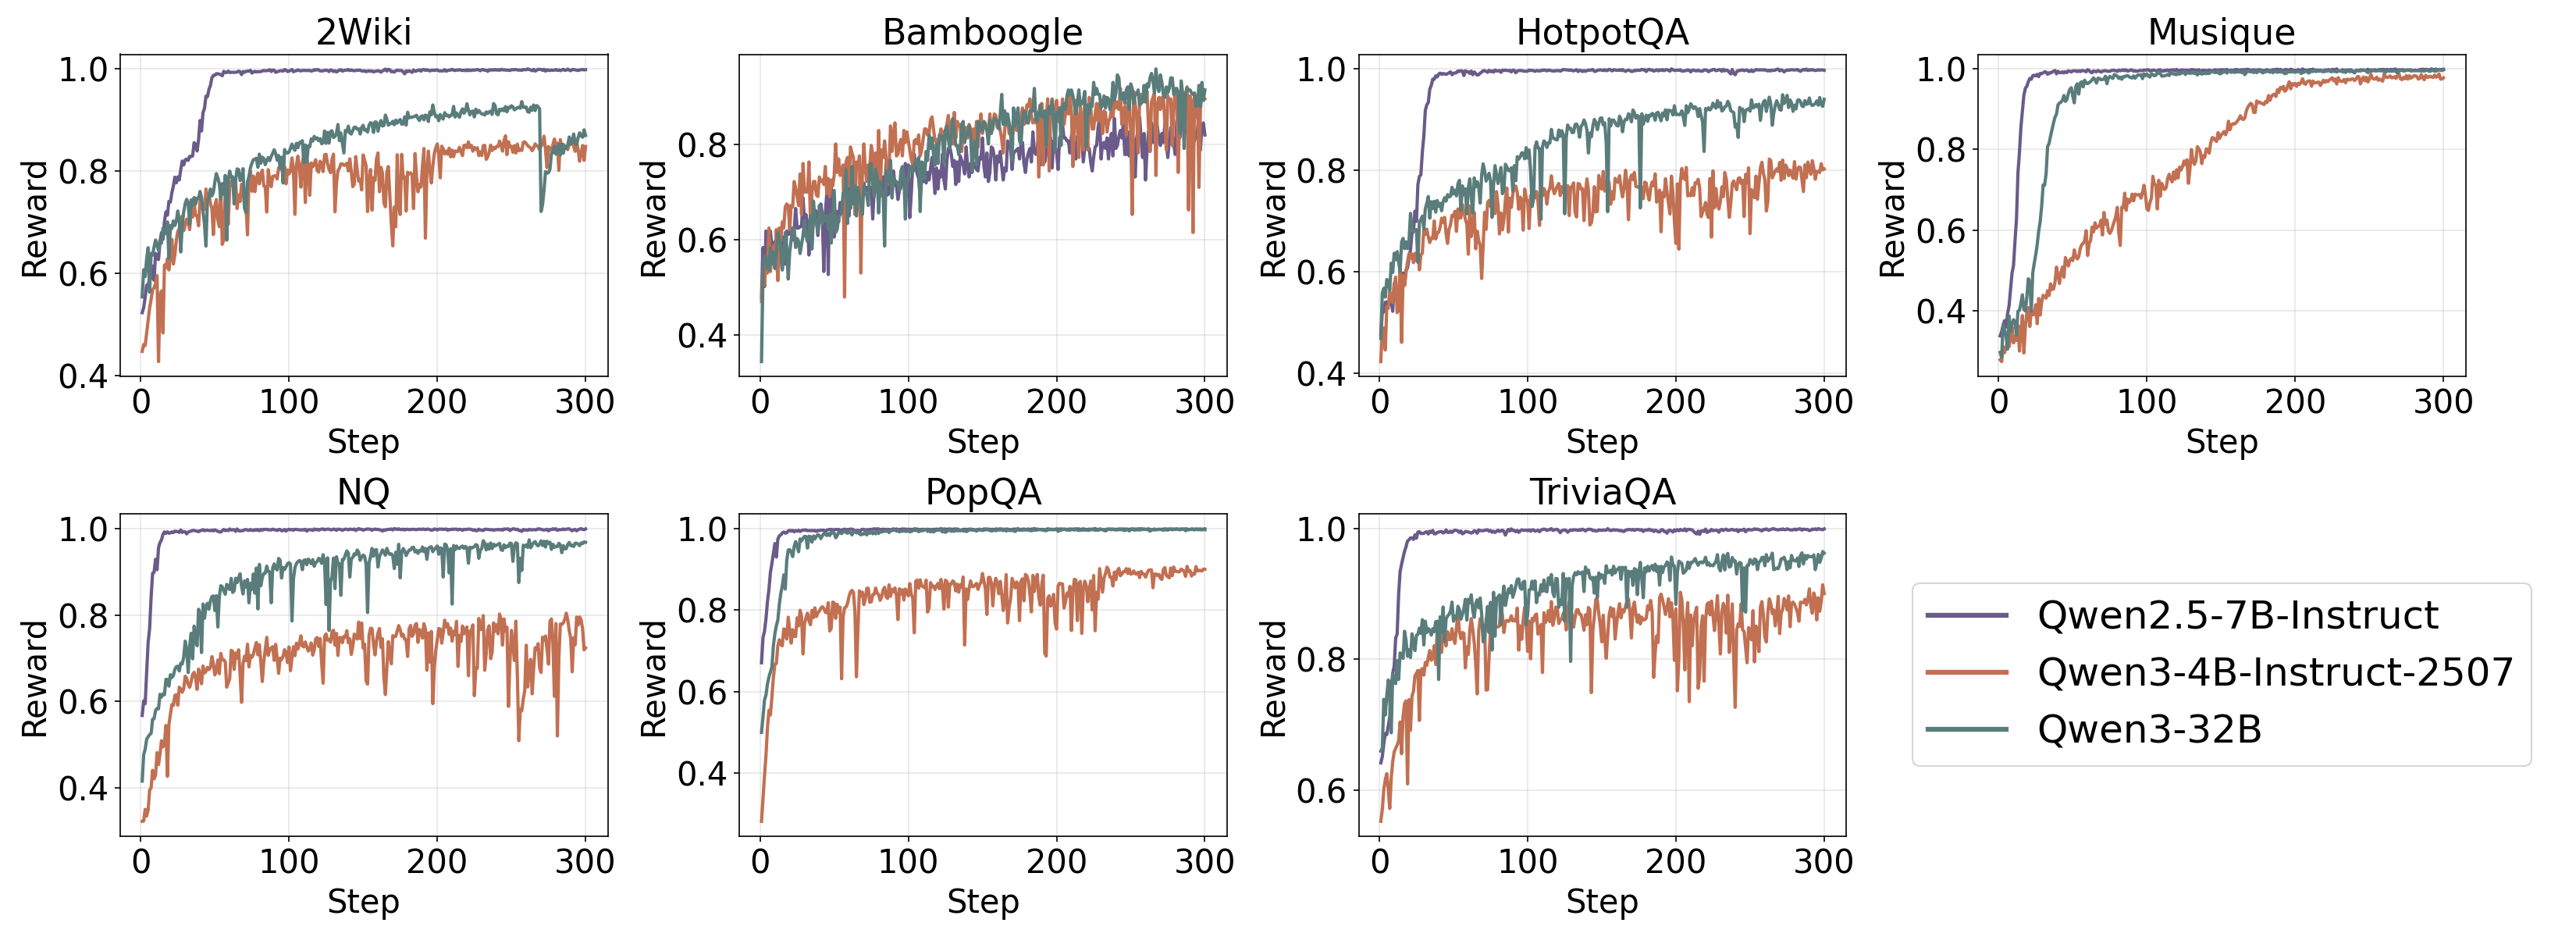
\includegraphics[width=1\linewidth]{img/ttrl_training_reward.png}
\caption{\textbf{Training reward for TTRL.}}
\label{fig:ttrl_train_reward}
\end{figure}



% \paragraph{Constitutional Judge (CJ)}
% ### Dimension 1: Response Quality
% Did the response address the user's actual underlying goal? Is it accurate, and appropriately scoped?
% Score 1 if poor, 5 if excellent.

% ### Dimension 2: Search Progression
% Did the agent's search queries progress appropriately across rounds?
% Score 1 if poor, 5 if excellent.

% ### Dimension 3: Evidence Synthesis
% Was the information accumulated across all search rounds accurately and fully reflected in the response?
% Score 1 if poor, 5 if excellent.
\paragraph{Constitutional Judge (CJ)}
Drawing on prior work in the interactive information retrieval literature \citep{borlund2003iir, kelly2009methods, carterette2011system}, we identify three core dimensions for evaluating multi-hop interactive information retrieval systems: \textit{Response Quality}, which assesses whether the final response addresses the user's underlying information need, is factually accurate, and is appropriately scoped; \textit{Search Progression}, which evaluates whether the agent's queries develop coherently and appropriately across successive steps; and \textit{Evidence Synthesis}, which measures whether information gathered throughout the search process is accurately integrated and fully reflected in the final response. Based on these dimensions, we design the prompt for the judge model. All other hyperparameters are identical to those described in \Cref{appendix:hyperparams}.


\paragraph{RLIF}
We compute the self-certainty metric for the final response in the entire search trajectory, as defined in Equation (2) of \citet{rlif}, and use it as the reward. All other hyperparameters are identical to those described in \Cref{appendix:hyperparams}.



\section{Limitations and Future Work}
CCS demonstrates that cycle-consistency can serve as an effective training signal for search agents without gold supervision, while also opening several avenues for future work. A practical limitation of the current framework is the need for an additional reconstruction model to compute rewards. Although this overhead is small relative to the overall cost of RL training, improving the efficiency of this component or integrating it more tightly into policy optimization would further strengthen the scalability of the approach. Moreover, our formulation is developed in the context of knowledge-intensive question answering, where search trajectories can often be viewed as informative representations of user intent. Extending this idea to broader agentic settings remains an important direction for future work.



% \section{Disclosure of LLM Usage}
% We used large language models for evaluation purposes (LLM-as-a-judge). Specifically, Gemini 2.5 Flash was used for question-answer benchmark evaluation (\Cref{tbl:main}), and Gemini 2.5 Pro was used for DeepResearch task evaluation (\Cref{fig:deepresearch}). In addition, Claude Opus 4.5 was used in an editorial role to assist with manuscript refinement and the identification and correction of minor typographical errors. All LLM-assisted outputs were carefully reviewed and revised by the authors, who retain full responsibility for the content, accuracy, and conclusions of this work.